% $Id: TalCV.tex,v 1.14 2011-01-31 18:20:14 dtal Exp $

\documentclass[conference,lettersize,twocolumn,twosize]{./IEEEtran}

% some very useful LaTeX packages include:

\usepackage{cite}

\usepackage[pdftex]{graphicx}
\graphicspath{{.}}

% \usepackage{subfigure}

\usepackage{url}

\usepackage{amsmath}

\usepackage[pdftex,hypertexnames=false]{hyperref}

% correct bad hyphenation here
\hyphenation{}

%%%%%%%%%%%%%%%%%%%%%%%%%%%%%%%%%%%%%%%%%%%%%%%%%%%%%%%%%%%%%%%%%%%%%%%%%%%%%%%

\begin{document}
\pagestyle{empty}
\section*{\bf \large{DORON TAL -- Curriculum Vitae}}
\subsection*{}
\begin{center}
  {\tt dt97@cornell.edu}\\
  {\tt \bf https://www.linkedin.com/in/mountainbot}\\
\end{center}
\subsection*{EDUCATION}
\begin{center}
  \begin{itemize}
  \item{{\bf Ph. D.}, \emph{Boston University}.
    Department of Cognitive and Neural Systems.  Mentor: Eric
    L. Schwartz, Computational Vision and Robotics Laboratory}
  \item{{\bf M. Eng.}, \emph{Cornell University}.
    Department of Computer Science.  Mentor: Alberto M. Segre,
    Artificial Intelligence Laboratory}
  \item{{\bf B. A.}, \emph{Cornell University}.
    Majors: Computer Science \& Philosophy. Minor: Cognitive
    Studies}
  \end{itemize}
\end{center}
\subsection*{SELECTED PROJECTS}
\begin{center}
  \begin{itemize}
  \item{\emph{Rapid learning in four legged robot locomotion
      policies}: Automatically teach a robot to walk, first in
    simulation, then in real life. Also used machine learning to (a)
    evaluate physical robot designs according to performance in
    simulation, (b) to automatically learn servo-couplings that work
    best for these robots (NASA Ames. Videos:
    \href{https://www.youtube.com/watch?v=nOca5QXBuTQ}{1},
    \href{https://www.youtube.com/watch?v=\_Dw67QpAlhU}{2}, 
    \href{https://www.youtube.com/watch?v=rp31BvijiqU}{3}
    ).}
  \item{3D camera localization using vision-based simultaneous
    localization and mapping}: Robot 3D localization, with a single
    grayscale camera, a single light source, known terrain heights and
    albedos and an Extended Kalman Filter (NASA Ames.
    \emph{\href{https://www.youtube.com/watch?v=zmq\_9Zw\_Awo)}{Video}
      ).}
  \item{\emph{Two dimensional image segmentation}: Partitioning an
    image into parts of homogeneous color or texture - implemened UC
    Berkeley's Normalized Cuts algorithm as an open source library,
    extended the algorithm to include color as a cue. Helped compile a
    database of human image segmentations.}
  \item{\emph{A simple biological model of neuron arithmetic}: Using
    the Integrate And Fire circuit for a model of a neuron we showed
    how, by modifying the refractory period of a neuron or its time
    constant, the neuron can shift its behavior from adding its inputs
    to multiplying them.}
  \item{\emph{Neural circuit for image segmentation}:
    my thesis has a model that ascribes the orientation singularities
    observed in visual cortex a function: image segmentation. Simple
    blurring of the input image edge response produces orientation
    singularities that segment the image into parts. We postulate that
    in the brain these orientation singularities form and change in
    response to an onchanging input-image and that they
    topographically represent segmented surfaces in the image, plus
    their shape.}
  \end{itemize}
\end{center}
\subsection*{EMPLOYMENT HISTORY}
\begin{center}
  \begin{itemize}
  \item{Sr. Research Engineer, {\bf Cornell Tech} Dec. 2017 - Present
    \emph{(1) Built the Cornell Tech Directory App for people to find
      out about each other - this included an API server with its
      database (EC2 node), and a client-app static file server (S3
      bucket). It was implemented in Ionic / Angular / Typescript for
      the client with Django REST Framework and PostgreSQL on the
      server; (2) Implemented computer vision algorithms to recognize
      and estimate the pose of a Lego brick (Python \& OpenCV); (3)
      Built a video portal to connect two places far apart with
      cameras, projectors and Raspberry Pi boards (Linux / Python /
      OpenCV). Co authored three, accepted, publications related to
      these projects.}}
  \item{President, {\bf Tracktunes, Inc.} Jul. 2013 - Present.  \emph{
      Tracktunes, Inc. is a benefit corporation devoted to building
      technology that help performing and composing musicians find
      each other, collaborate, share and sell music. }}
  \item{Sr. Vision Scientist, {\bf Videosurf, Inc.}  (acquired by \bf
    Microsoft}). August, 2007 - October, 2010.  \emph{Computer vision
    algorithms for video search, facial pose estimation and object
    segmentation out of videos; text entity extraction and automatic
    tagging of video data with Freebase articles and relationships.}

  \item{Computer Vision Research Scientist, {\bf Paravue, Inc.},
    Oakland, CA.  February, 2007 - August, 2007.  \emph{Fast image
      segmentation algorithms on megapixel images, for automatic
      clipping of objects from images for later labeling and for
      Paravue's Turbomask (TM) Adobe Photoshop auto-clipping plugin}.}
  \item{Research Scientist, USRA/RIACS at {\bf NASA Ames Research
      Center}, Moffett Field, CA.  March, 2002 -- April, 2006.
    \emph{3D vision based SLAM (
      \href{https://www.youtube.com/watch?v=zmq\_9Zw\_Awo)}{Video}). Combined
      robotics with computer vision for mapping and localization;
      implemented stereo vision and camera calibration for Autonomous
      Rotorcraft Project on UAV's hardware; interfaced the UAV's
      sensors to a reactive planner for automatic machine diagnostics;
      machine learning for robot controller symmetry optimization;
      machine learning for automatic robot design; articulated robot
      physics based simulation used ODE, Open Inventor and accurate
      friction models for ground-foot interaction; built second
      quadruped robot``RTQ''}.}
  \item{Director, {\bf VisBot}, Inc. Berkeley, CA.  August, 2001 --
    August, 2003.  \emph{Built first quadruped prototype and taught it
      various walking gaits with Andrew Ng and Greg Williams at UC
      Berkeley}.}
  \item{Postdoctoral Fellow, NIH funded, Vision Group at {\bf
      University of California, Berkeley}, CA. February, 2000 -- June,
    2001.  \emph{Image segmentation with Jitendra Malik, implemented
      the ``Normalized Cuts'' algorithm and augmented it with color
      processing capability, developed metrics for benchmarking both
      human and machine segmentations of images}.}
  \item{Research Scientist and founding member, {\bf Visionics
      Corporation}. Jersey City, NJ. July, 1997 -- January,
    2000. \emph{Face detection, high-accuracy face alignment,
      tracking moving heads, low level image processing and
      enhancement for face recognition.  Visionics is known today as
      ``L1 Identity Solutions, Inc.''}.}
  \item{Postdoctoral Fellow, {\bf Mount Sinai School of
      Medicine}. Neuroscience Laboratory. New York, NY. September,
    1997 -- June, 1997. \emph{Optical imaging in striate cortex of cat
      and monkey, and pattern recognition in optical imaging data}. }
  \item{Research Assistant, {\bf Boston University, Department of
      Cognitive and Neural Systems, Computational Vision and Robotics
      Laboratory}. September, 1993 -- January, 1997. \emph{Graduate
      Research: (1) human and animal segmentation of visual imagery;
      (2) a model of how neurons can either multiply or add their
      inputs, depending on two common parameters; (3) structure and
      function of vortex formation in mamallian brains.}}
  \item{Research Engineer, {\bf Xerox Corporation -- Rochester
      Research Center}, Rochester, NY. January 1992 -- July,
    1992. \emph{Co-author of "ask", Xerox's natural language company
      information database program}.}
  \end{itemize}
\end{center}
\subsection*{SELECTED PUBLICATIONS}
\begin{itemize}
\item{Tal, D. (2006).  Evaluating symmetry variations in quadruped
  trot gait locomotion controllers.  \emph{IEEE International Conference
    on Robotics and automation: Submitted to ICRA '07}.}
\item{Lutz R., Patterson-Hine A., Nelson S., Frost C. R., Tal D. and
  Harris, R. (2006).  Using Obstacle Analysis to Identify
  Contingency Requirements on an Unpiloted Aerial Vehicle.
  \emph{Requirements Engineering Journal}, Springer Verlag.
  \emph{Accepted Sept., 2006}.}
\item{Tal, D. (2005).  Robot and Locomotion-Controller Design
  Optimization for a Reconfigurable Quadruped Robot.  Universities
  Space Research Association Technical Report 05-29.}
\item{Lutz R., Patterson-Hine A., Nelson S., Frost C. R. and Tal
  D. (2005).  Identifying Contingency Requirements Using Obstacle
  Analysis. \emph{13th IEEE Requirements Engineering Conference
    2005}.}
\item{Tal D. and Malik J. (2001).  Combining Color, Texture and
  Contour for Image Segmentation.  Technical Report , UC Berkeley
  Computer Science Department.}
\item{Martin D., Fowlkes C., Tal D. and Malik J. (2001). A database
  of human segmented natural images and its application to
  evaluating segmentation algorithms and measuring ecological
  statistics. \emph{ ICCV} 2001. }
\item{Tal D. and Schwartz E. L. (1997).  Topological singularities
  in cortical orientation maps: the sign theorem correctly predicts
  orientation column patterns in primate striate cortex
  \emph{Network: Computation in Neural Systems} {\bf 8}(2),229-238.}
\item{Tal D. and Schwartz E. L. (1997).  Computing with the leaky
  integrate and fire model: logarithmic computation and
  multiplication.  \emph{Neural Computation} {\bf 9},305-318.}
\item{Tal D. and Schwartz E. L. (1996).  Statistical analysis and
  parametrization of experimental and theoretical vortex maps in
  primate striate cortex (oral presentation).
  \emph{Invest. Opthal. \& Vis. Sci. Suppl.} {\bf 37}(3), 938.}
\item{Tal D. and Schwartz E. L. (1995). Computing with the integrate
  and fire neuron: Multiplication, addition and phase
  detection. \emph{ Technical Report} CAS/CNS-95-024, Boston
  University.}
\item{Tal D. and Schwartz E. L. (1994).  Weber-Fechner transduction
  -- a logarithmic compressive nonlinearity is a generic property of
  integrate and fire neurons (paper presentation).
  \emph{Proceedings of the INNS World Congress on Neural Networks.}
       {\bf IV}, 350.}
\item{Gaudiano P., Olson S., Tal D., and Fischl B. (1993). A neural
  network model of dynamic receptive field
  reorganization. \emph{Society for Neuroscience Abstracts}, {\bf
    19} (1), 809.}
\end{itemize}
\subsection*{SOFTWARE}
\begin{itemize}
\item{Hybrid web apps. Music collaboration and recording
  app. (HTML/CSS/Javascript/Ionic/Angular/Python/Postgres/AWS).
  Tracktunesd Inc and others, 2013-2018.}
\item{Textual data mining and analysis - matching any phrase in
  YouTube video description text with Wikipedia page titles: if there
  is an unambiguous match, we turn the phrase in the video description
  into a link to the Wikipedia article. Videosurf Inc, 2010.}
\item{The Normalized Cuts image segmentation algorithm (C++, Matlab).
  University of California at Berkeley, Department of Computer
  Science, 2000.}
\item{Face tracking and head alignment algorithms (Matlab, C++),
  Visionics Inc., 1997.}
\end{itemize}
% \vspace{1in}
\subsection*{HARDWARE}
\begin{itemize}
\item{Yellowbot: Built in collaboration with Andrew Ng and Gregory
  Williams at UC Berkeley to test machine learning algorithms for
  quadruped walking.  In 2003, it was donated to Stanford's robotics
  lab.  (Videos: \href{https://www.youtube.com/watch?v=nOca5QXBuTQ}{1},
  \href{https://www.youtube.com/watch?v=\_Dw67QpAlhU}{2}, 
  \href{https://www.youtube.com/watch?v=rp31BvijiqU}{3})}
\end{itemize}
\begin{figure}[ht]
  \centering      
  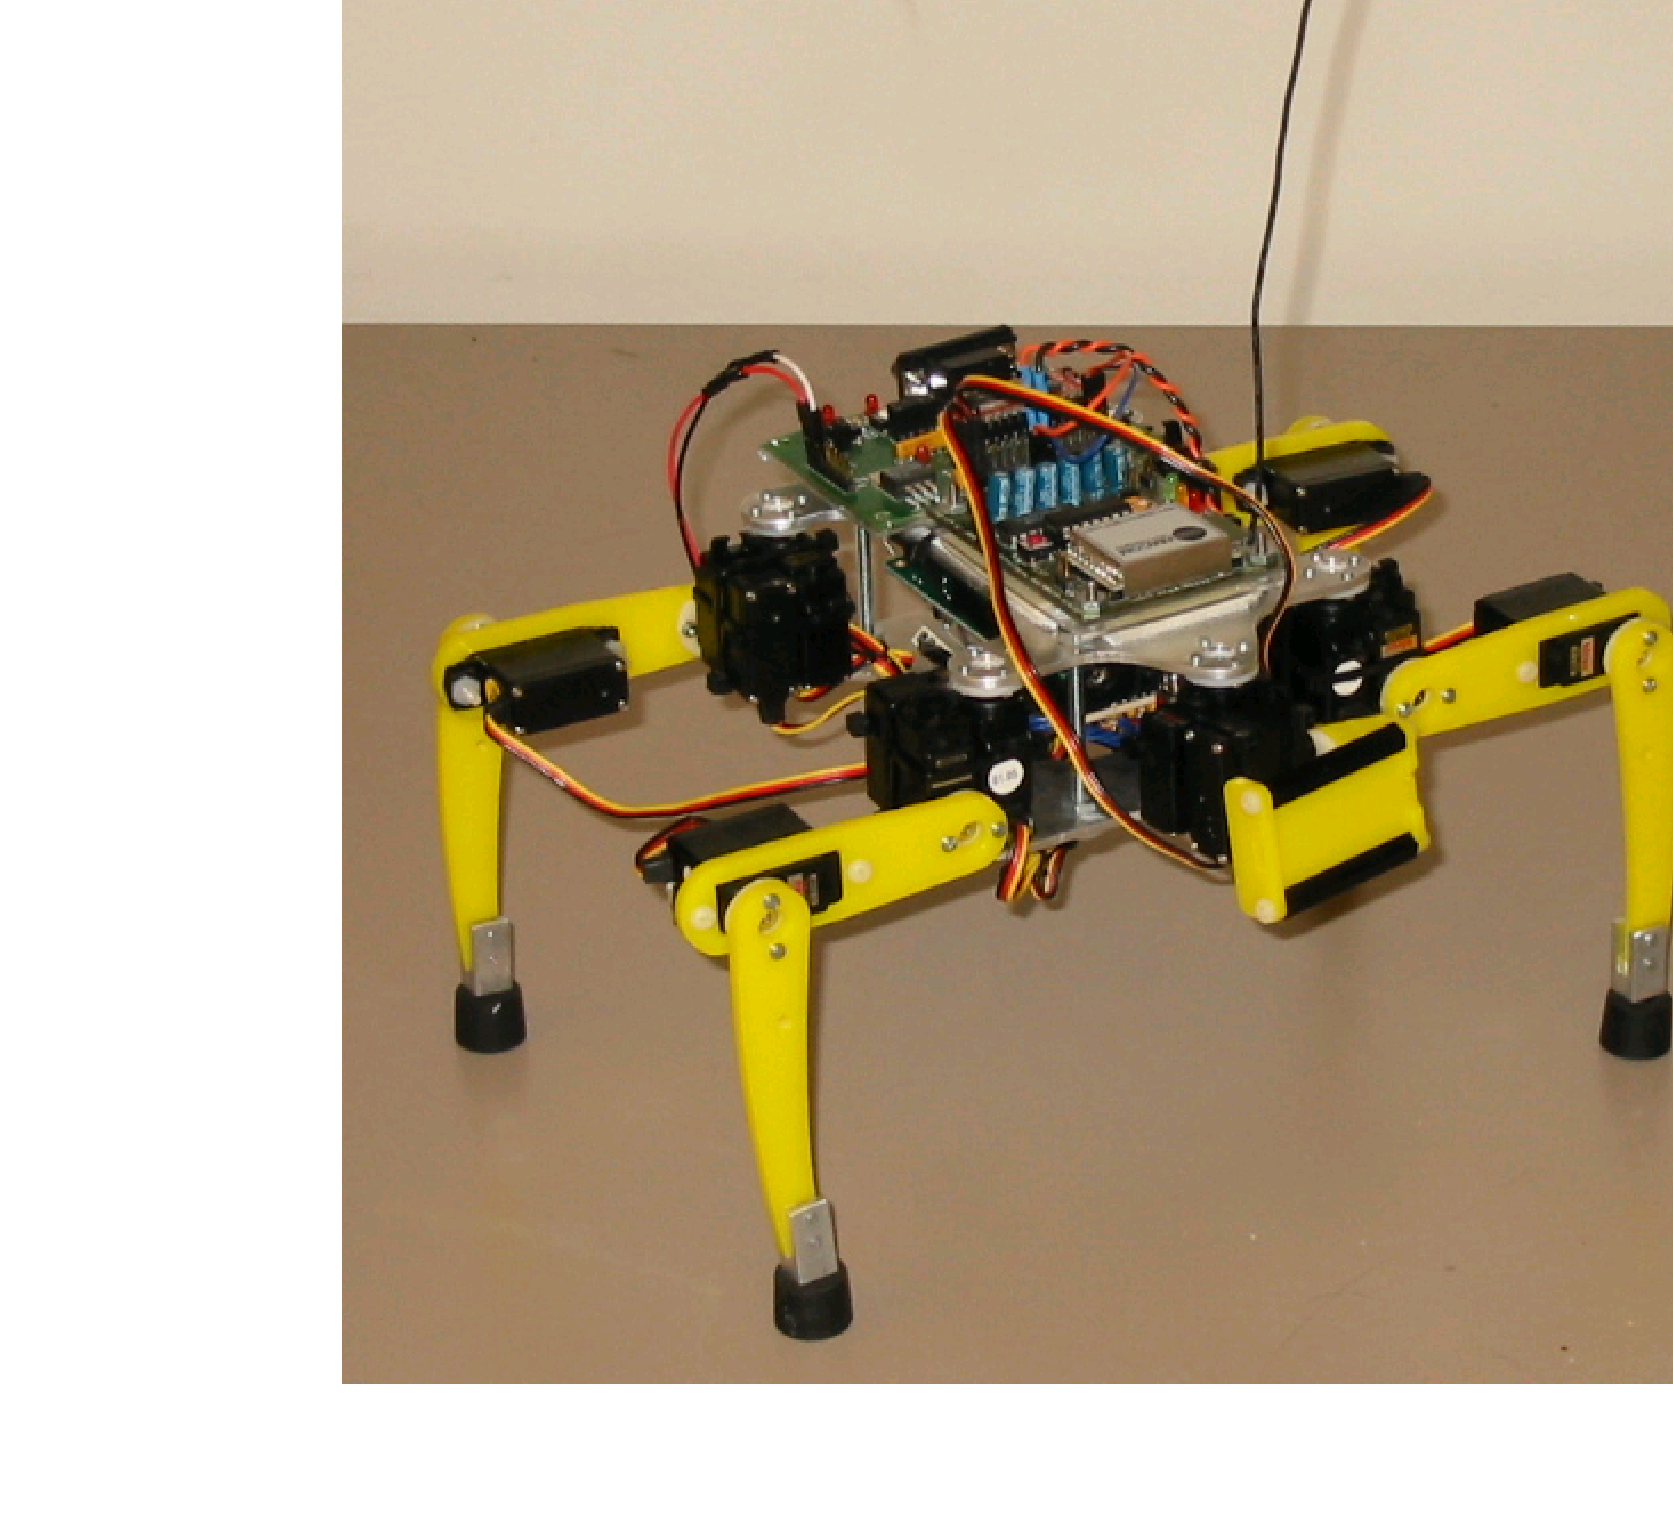
\includegraphics[height=0.5in,width=0.5in]{yellowbot.pdf}
\end{figure}
\begin{itemize}
\item{Rough Terrain Quadruped (RTQ): First outdoor version, developed
  at NASA Ames Research Center.  This robot is physically symmetric
  along front/hind, left/right up/down axes. It has many improvements
  in durability and weight reduction over yellowbot.}
\end{itemize}
\begin{figure}[ht]
  \centering      
  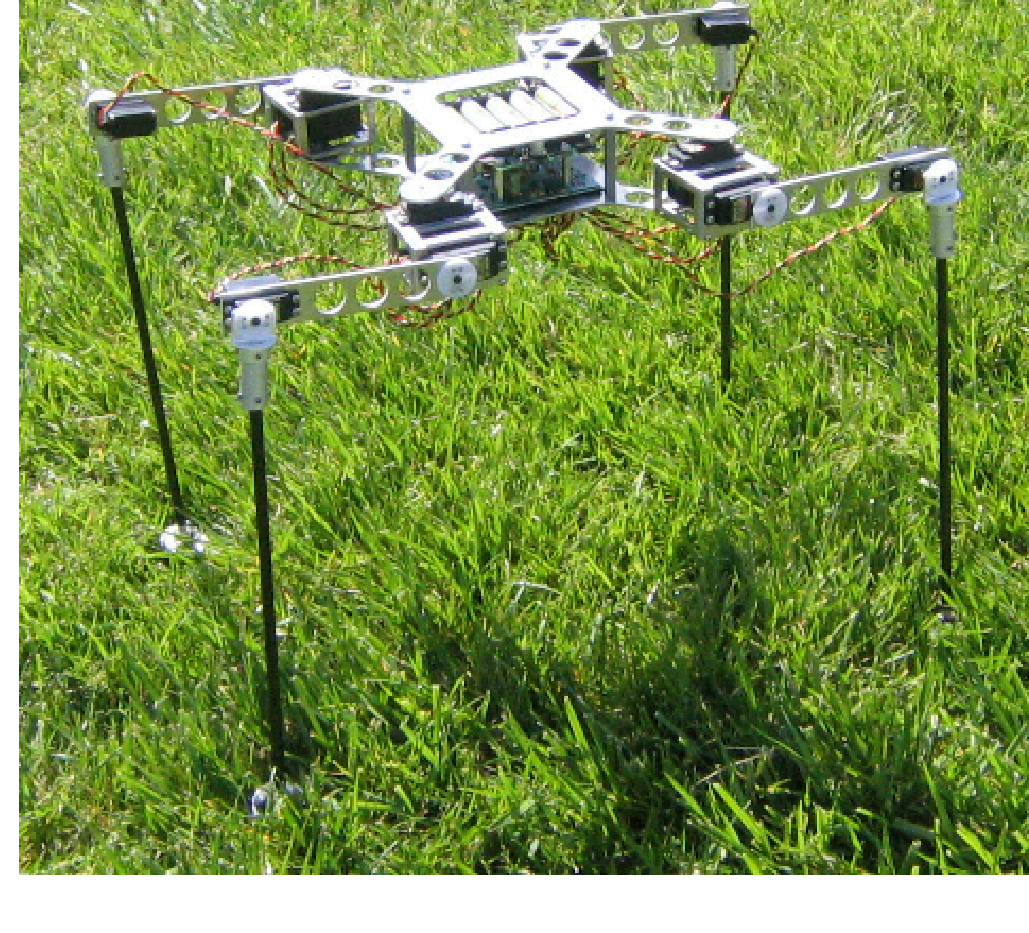
\includegraphics[height=0.5in,width=0.5in]{rtq.pdf}
\end{figure}
\begin{itemize}
\item{Rough Terrain Quadruped II (RTQ2).  Further physical
  improvements: stronger lower legs, spring-suspension lower-leg
  shocks and a water-sealed box for power and electronics.}
\end{itemize}
\begin{figure}[ht]
  \centering      
  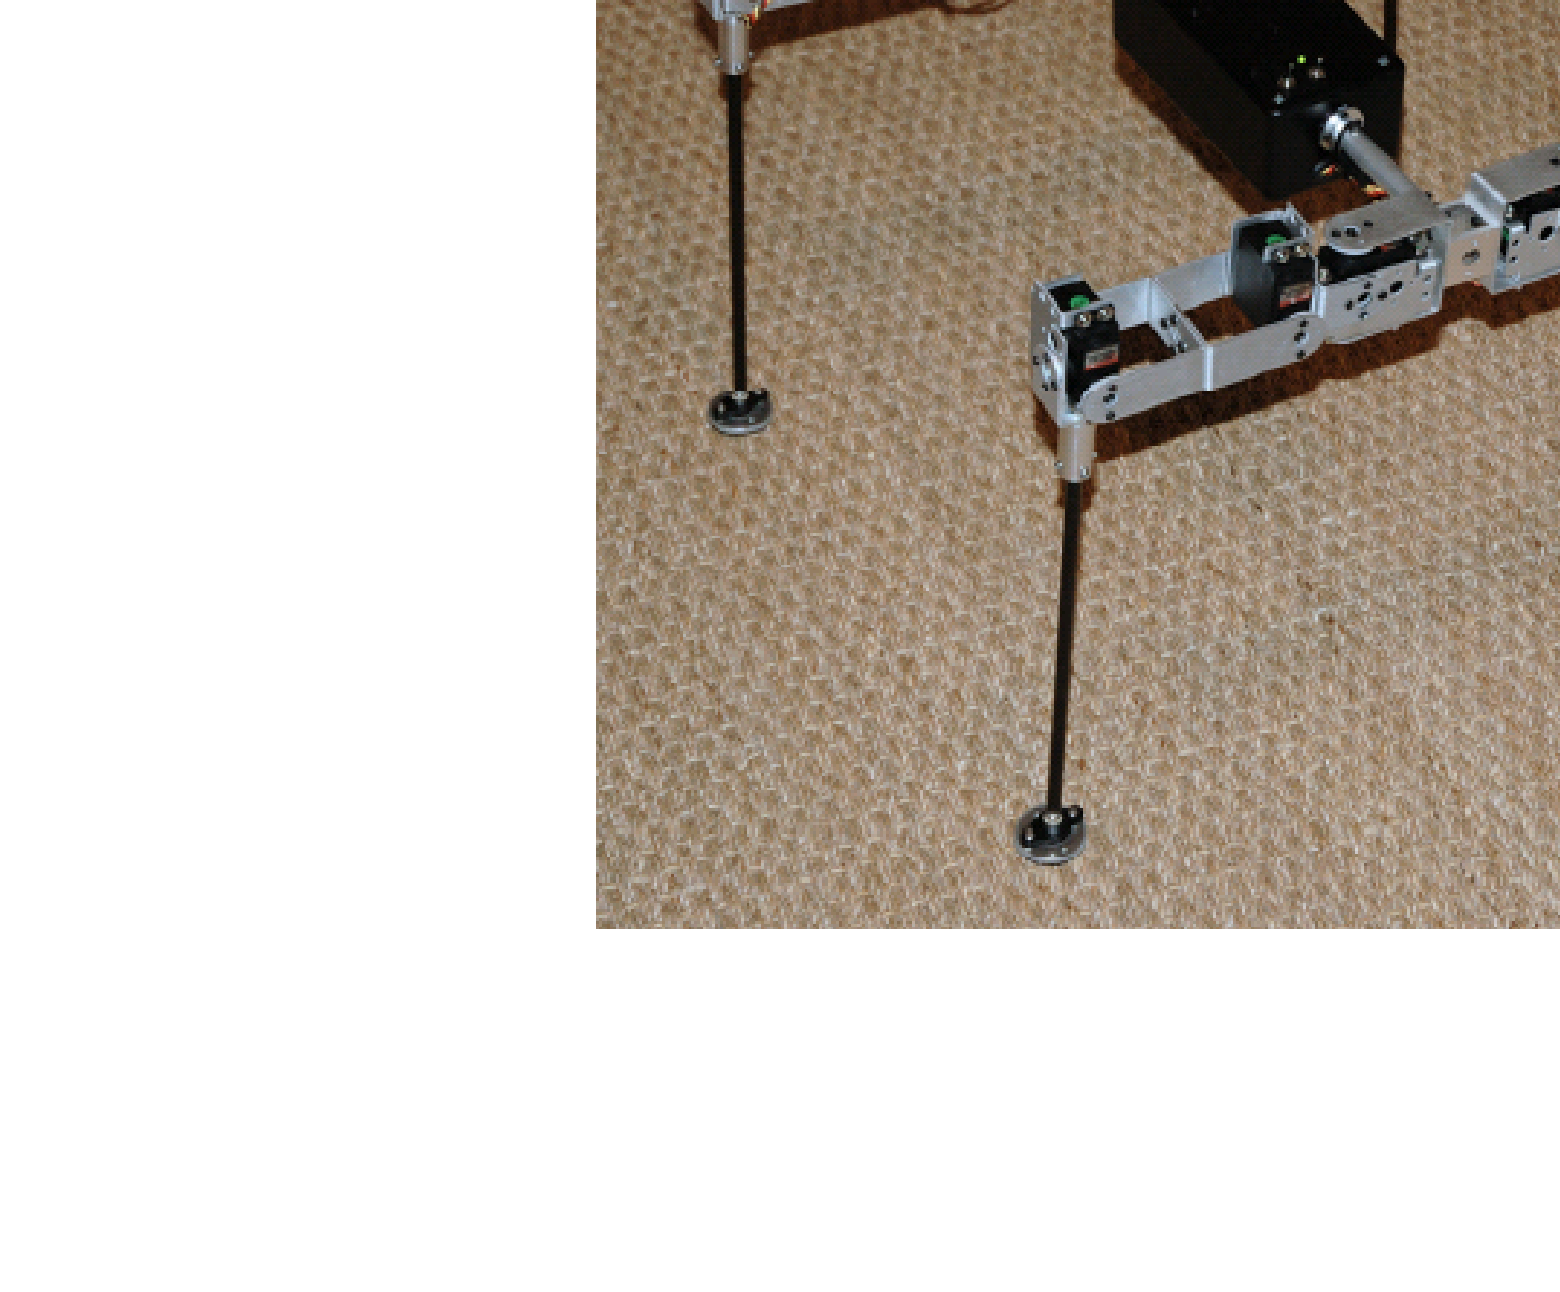
\includegraphics[height=0.5in,width=0.5in]{mountainbot.pdf}
\end{figure}
\end{document}
\tt
